%!TEX root = ../../thesis.tex
\section{Drum Machine}
\label{impl-drum-machine}

\begin{lstlisting}[language=JavaScript, caption=A drum machine's data structure, label=lst:drum-structure]
  {
    "type": "drum",
    "position": 0.78,
    "drumType": "808",
    "patternOrder": ["a","b"],
    "patterns": { a: Object, b: Object (...) }
  }
\end{lstlisting}

A drum machine piece is made of a meta data structure (\reflisting{lst:drum-structure}), which contains information about pattern order (line 5) and the drum kit type (line 4), and it also contains the information of all patterns (line 6).

\begin{lstlisting}[language=JavaScript, caption=A pattern's data structure, label=lst:pattern-structure]
  {
    "bpm": 70,
    "slots": 8,
    "beats": {
      "bass":  [1,0,0,0,0,0,0,0],
      "snare": [0,0,0,0,1,0,0,0]
      (...)
    }
  }
\end{lstlisting}

Patterns are the core data structure (\reflisting{lst:pattern-structure}) that contain the information about playback speed (line 2) and the beat order (line 5f). A value of \code{1} in one of the beat arrays means, that a beat will be played at this index. For example, the \code{snare} will only be played it index 5 (line 6). The \code{slots} property defines the length of the beat arrays. When the values is changed by the user, the arrays will either get cut off from the end (\code{slot} has been reduced) or they will be filled up with zeros (\code{slot} has grown).

Patterns have been specifically designed to allow musicians to be as flexible as possible. One drum machine piece can contain six different patterns (a-f). These patterns will all have the same base drum kit. Each pattern can have a different speed and a different amount of slots. The playback order for the patterns of a drum machine is defined in the \code{patternOrder} property. The example in \reflisting{lst:drum-structure} has an order of \code{["a", "b"]}. So pattern \code{a} is the first pattern to be played and \code{b} will be played afterwards. In this way, a wide variety of complex drum patterns and rhythms can be achieved by using only a single drum machine piece.

The preview playback (as seen in \refchapter{fig:editor-editing-a-loop}) uses a simple algorithm to loop the pattern. It is based on a high-frequency \code{Ticker}, an object that ticks another function every 30ms.

\begin{lstlisting}[language=JavaScript, caption=A pattern's loop algorithm, label=lst:pattern-loop]
  if(shouldPlayNextBeat()){
    beat = beat + 1;
    if(beat >= slots) beat = 0;

    nextBeatTime += secondsBetweenBeats();

    for(instrument in instruments){
      if(beats[instrument][beat]){
        play(instrument, nextBeatTime);
      }
    }
  }
\end{lstlisting}

For each tick, the algorithm first checks if a new beat should be played (line 1, \reflisting{lst:pattern-loop}). The method simply checks if the current time and the calculated time for the next beat overlap. Next, the current \code{beat} needs to be increased (line 2) and if the \code{beat} is the same size as the \code{slot} property, which defines the length of a pattern, it is reset to \code{0} so that the pattern starts over when its end has been reached (line 3). The exact time for the next beat is calculated by adding the amount of seconds per beat to the last time a beat has been played (line 5). The amount of seconds is calculated from the pattern's BPM. In the last step, the algorithm iterates over all instruments\footnote{Instruments here stand for the individual parts of a drum kit e.g. `hihat' or `snare drum'.} and checks if it should be played at the current beat\footnote{The current beat is the same as the beat index from line 5 of \reflisting{lst:pattern-structure}} (line 7ff). In the `global' playback, another scheduling algorithm is used for  performance reasons, which is explained in \refchapter{sec:impl-scheduling}.

There are several different drum machines from which users can choose. Each consisting of four to eight different instruments. So normally this would mean that for each drum kit that is used in an arrangement HTTP GET requests are started to load each instrument individually. In a case where an arrangement contains a lot of different drum kits, a lot of HTTP requests would be created which would slow down the application start. Thus, another technique is used to load drum kits: Audio sprites.

\begin{figure}[htb]
  \centerline{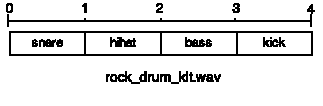
\includegraphics[width=0.9\linewidth]{images/drumkit_wav.pdf}}
  \caption[Audiosprites visualized]{Audiosprites visualized}
  \label{fig:audiosprites}
\end{figure}

The aim of audio sprites is to reduce the overall amount of HTTP requests, because they create an immense communication overhead. A benchmark\footnote{\url{http://janmonschke.com/Master-Thesis-Project/experiments/audio-sprites-benchmark/}, last checked on 21/03/2014} has shown\footnote{The test was executed from the same computer 10 times for each method in three different wirelesse networks. Caching was disabled while the tests ran.} that audio sprites reduce the load time by up to 50\% (see results in \refchapter{ch:speed-comparison}). Based on these results, all drum kits were implemented as audio sprites.

Audio sprites combine all individual audio files into one single large file. They also provide information about the position of the individual audio files into the one large file. As seen on \reffigure{fig:audiosprites}, the file \code{rock\_drum\_kit.wav} contains a \code{snare}, a \code{hihat}, a \code{bass} and a \code{kick} audio file. Each file is one second long\footnote{The real audio sprites leave some miliseconds pause between each individual file, so that there can be no overlapping audio data. For the sake of simplicity, these pauses are not shown in \reffigure{fig:audiosprites}}. The audio sprite for this drum kit would then contain the following offset information: \code{snare: [0, 1], hihat: [1, 2] (...)}. In the implementation, a drum kit is represented by one single buffer file (compare \refchapter{sec:webaudio-buffer}) and each time an instrument needs to be played, this buffer and the instrument's offset information are used to play the correct part of the drum kit's buffer (compare \refchapter{subsec:timing-in-web-audio}).